\begin{frame}{Group Theory to the rescue!}
  \begin{block}{Definition}
    A \textbf{group} $(G, *)$ is a set closed under the multiplication $*$, together with the existence of unique inverse elements.
  \end{block}
    {\small Example: The set of all bijections of the set $\{1,\ldots n\}$ with composition is a group (known as the full symmetric group on $n$ letters $S_n$).}
    
    $S_2 = \{(1)(2), (1,2)\}$ \textbf{acts} on polynomial ring $\mathbb{R}[x]$ by
    \begin{align*}
      ((1)(2), x) & \mapsto x\\
      ((1, 2), x) & \mapsto -x.
    \end{align*}
    {\small Observe: $f(x) = x^4 - 2x^2$ is invariant under this action.\\
    Observe: $f(x) = x^6 - 2x^4 + 2x^2 = x^2 + (x-x^3)^2$ is invariant, but one of the summands isn't!}
    
\end{frame}


\begin{frame}{Isotypical projections}
    ``Types'' of actions $\leftrightarrow$  blocks in the block-diagonalization:
    \[V \cong V_1 \oplus \cdots \oplus V_k.\]
    
    Each block $V_i$ decomposes further as 
    $V_i = \oplus_{m_i} V_i'$. (\footnote{$m_i$ is the multiplicity of the action type in $V$})
    
    Universal (baseless) projections\footnote{related to irreducible characters} in \textbf{group ring $\mathbb{R}[G]$} $\leftrightarrow$ projections onto blocks (for every $V$!).
%     
    \begin{block}{Example}
    \small
    Universal projections for $S_2$:\\[-0.2in]
    \begin{align*}
      p_1 = \frac{1}{2}((1)(2) + (1,2)) & \to\text{invariants}\\ 
      p_2 = \frac{1}{2}((1)(2) - (1,2)) & \to\text{flipped}
    \end{align*}
    \end{block}
    
\end{frame}

\begin{frame}[fragile]{Permutation symmetry example}
\footnotesize
\begin{minted}{julia}
  using DynamicPolynomials
  @polyvar x[1:4]
  f = sum(x) + sum(x.^2)

  using PermutationGroups
  G = PermGroup([perm"(1,2,3,4)"])
  # permutation group generated by one element (cyclic of order 4)

  basis = monomials(x, 0:(maxdegree(f)÷2))
  using SymbolicWedderburn
  symmetry_adapted_basis(G, basis, OnVariables())
  # G acts by permuting variables
\end{minted}

Isotypical blocks when acting on $[1, x_1, x_2, x_3, x_4, x_5]$:
\[
  B_1 = \begin{bmatrix}
          1\\
          x_1 + x_2 + x_3 + x_4
        \end{bmatrix}
  \qquad
  B_2 = \begin{bmatrix}
          x_1 - x_3\\
          x_2 - x_4
        \end{bmatrix}
  \qquad
  B_3 = \begin{bmatrix}
          x_1 - x_2 + x_3 - x_4
        \end{bmatrix}
\]
\end{frame}

\begin{frame}[fragile]{Permutation symmetry example}
\footnotesize
\begin{minted}{julia}
  using SumOfSquares
  import CSDP
  model = Model(CSDP.Optimizer)
  @variable(model, t)
  @objective(model, Max, t)
  con_ref = @constraint(model, poly - t in SOSCone(), 
      symmetry = SymmetryPattern(G, VariablePermutation())) 

  optimize!(model)
\end{minted}

\normalsize
Naive formulation $5\times 5$-sdp; symmetry adapted: $2\times 2$, $2\times 2$, $1\times 1$-sdps.

Note: the sizes here correspond to the multiplicities of irreducible subspaces, \textbf{not} their dimensions!

\end{frame}

\begin{frame}[fragile]{Even symmetry example}
\footnotesize
\begin{minted}{julia}
  struct OnSign <: OnMonomials end
  # <: SymbolicWedderburn.Action
  SymbolicWedderburn.action(::OnSign, p::Permutation, 
      mono::AbstractMonomial) = sign(p)^degree(mono)*mono
  # corresponds to x → -x
  
  G = PermGroup([perm"(1,2)"])
  
  @polyvar x
  f = x^6 - 2x^4 + 2x^2
  basis = monomials(x, 0:(maxdegree(f)÷2))
  symmetry_adapted_basis(G, basis, OnSign())  
\end{minted}

  Isotypical blocks when acting on $[1, x, x^2, x^3]$:
\[
  B_1 = \begin{bmatrix}
          1\\
          x^2
        \end{bmatrix}
  \qquad
  B_2 = \begin{bmatrix}
          x\\
          x^3
        \end{bmatrix}
\]

\end{frame}

\begin{frame}[fragile]{Dihedral symmetry example}
\footnotesize
  \begin{minted}{julia}
  @polyvar x y
  f = x^6 + y^6 - x^4 * y^2 - y^4 * x^2 - x^4 - y^4 - 
      x^2 - y^2 + 3x^2 * y^2 + 1
  struct DihedralAction <: 
      SymbolicWedderburn.ByLinearTransformation end
  \end{minted}
  The action is a mixture of changing sign and permuting variables.
  \begin{minted}{julia}
  import GroupsCore
  struct DihedralGroup <: GroupsCore.Group ... end
  struct DihedralElement <: GroupsCore.GroupElement
      ...
  end
  \end{minted}
  \begin{itemize}
    \item implement methods from \texttt{GroupsCore.jl} API for \texttt{DihedralGroup}
    \item implement action methods from \texttt{SymbolicWedderburn} for \texttt{DihedralAction}
  \end{itemize}


\end{frame}

\begin{frame}{Groups interface: \texttt{GroupsCore.jl}}
  ??? I don't think we will have time for this???
\end{frame}

\begin{frame}{Groups interface: \texttt{SymbolicWedderburn.jl}}
    Behind the scenes:
    \begin{itemize}
      \item compute \textbf{character table} of the group $\longrightarrow$ universal projections
      \item given action e.g. on monomials, \textbf{induce} the action to the whole basis
      \item evaluate the projections in the action $\longrightarrow$ \textbf{block diagonalizing} change of basis
      \item further \textbf{decompose} each block into to \textbf{irreducible} blocks\footnote{for now numerically only}.
    \end{itemize}
\end{frame}


\begin{frame}{Large scale example}

  \begin{itemize}
    \item Optimization problem from geometric group theory\footnote{Kaluba, M., Nowak, P.W. \& Ozawa, N. $\operatorname{Aut}(F_5)$ has property (T). \textit{Math. Ann}. \textbf{375}, 1169–1191 (2019). \url{https://doi.org/10.1007/s00208-019-01874-9}}
    \item sdp-constraint of size $4\,641\times 4\,641$, $~1.1\cdot 10^7$ constraints
    \item symmetry group: $S_2 \wr S_5$ ($3840$ elements)
    \item After symmetrization:
      \begin{itemize}
          \item $36$-blocks (largest: $58\times 58$), $13\,232$ variables in total
          \item $7\,230$ constraints
      \end{itemize}
    \item Solvable!    
  \end{itemize}

\end{frame}

\begin{frame}
\centering
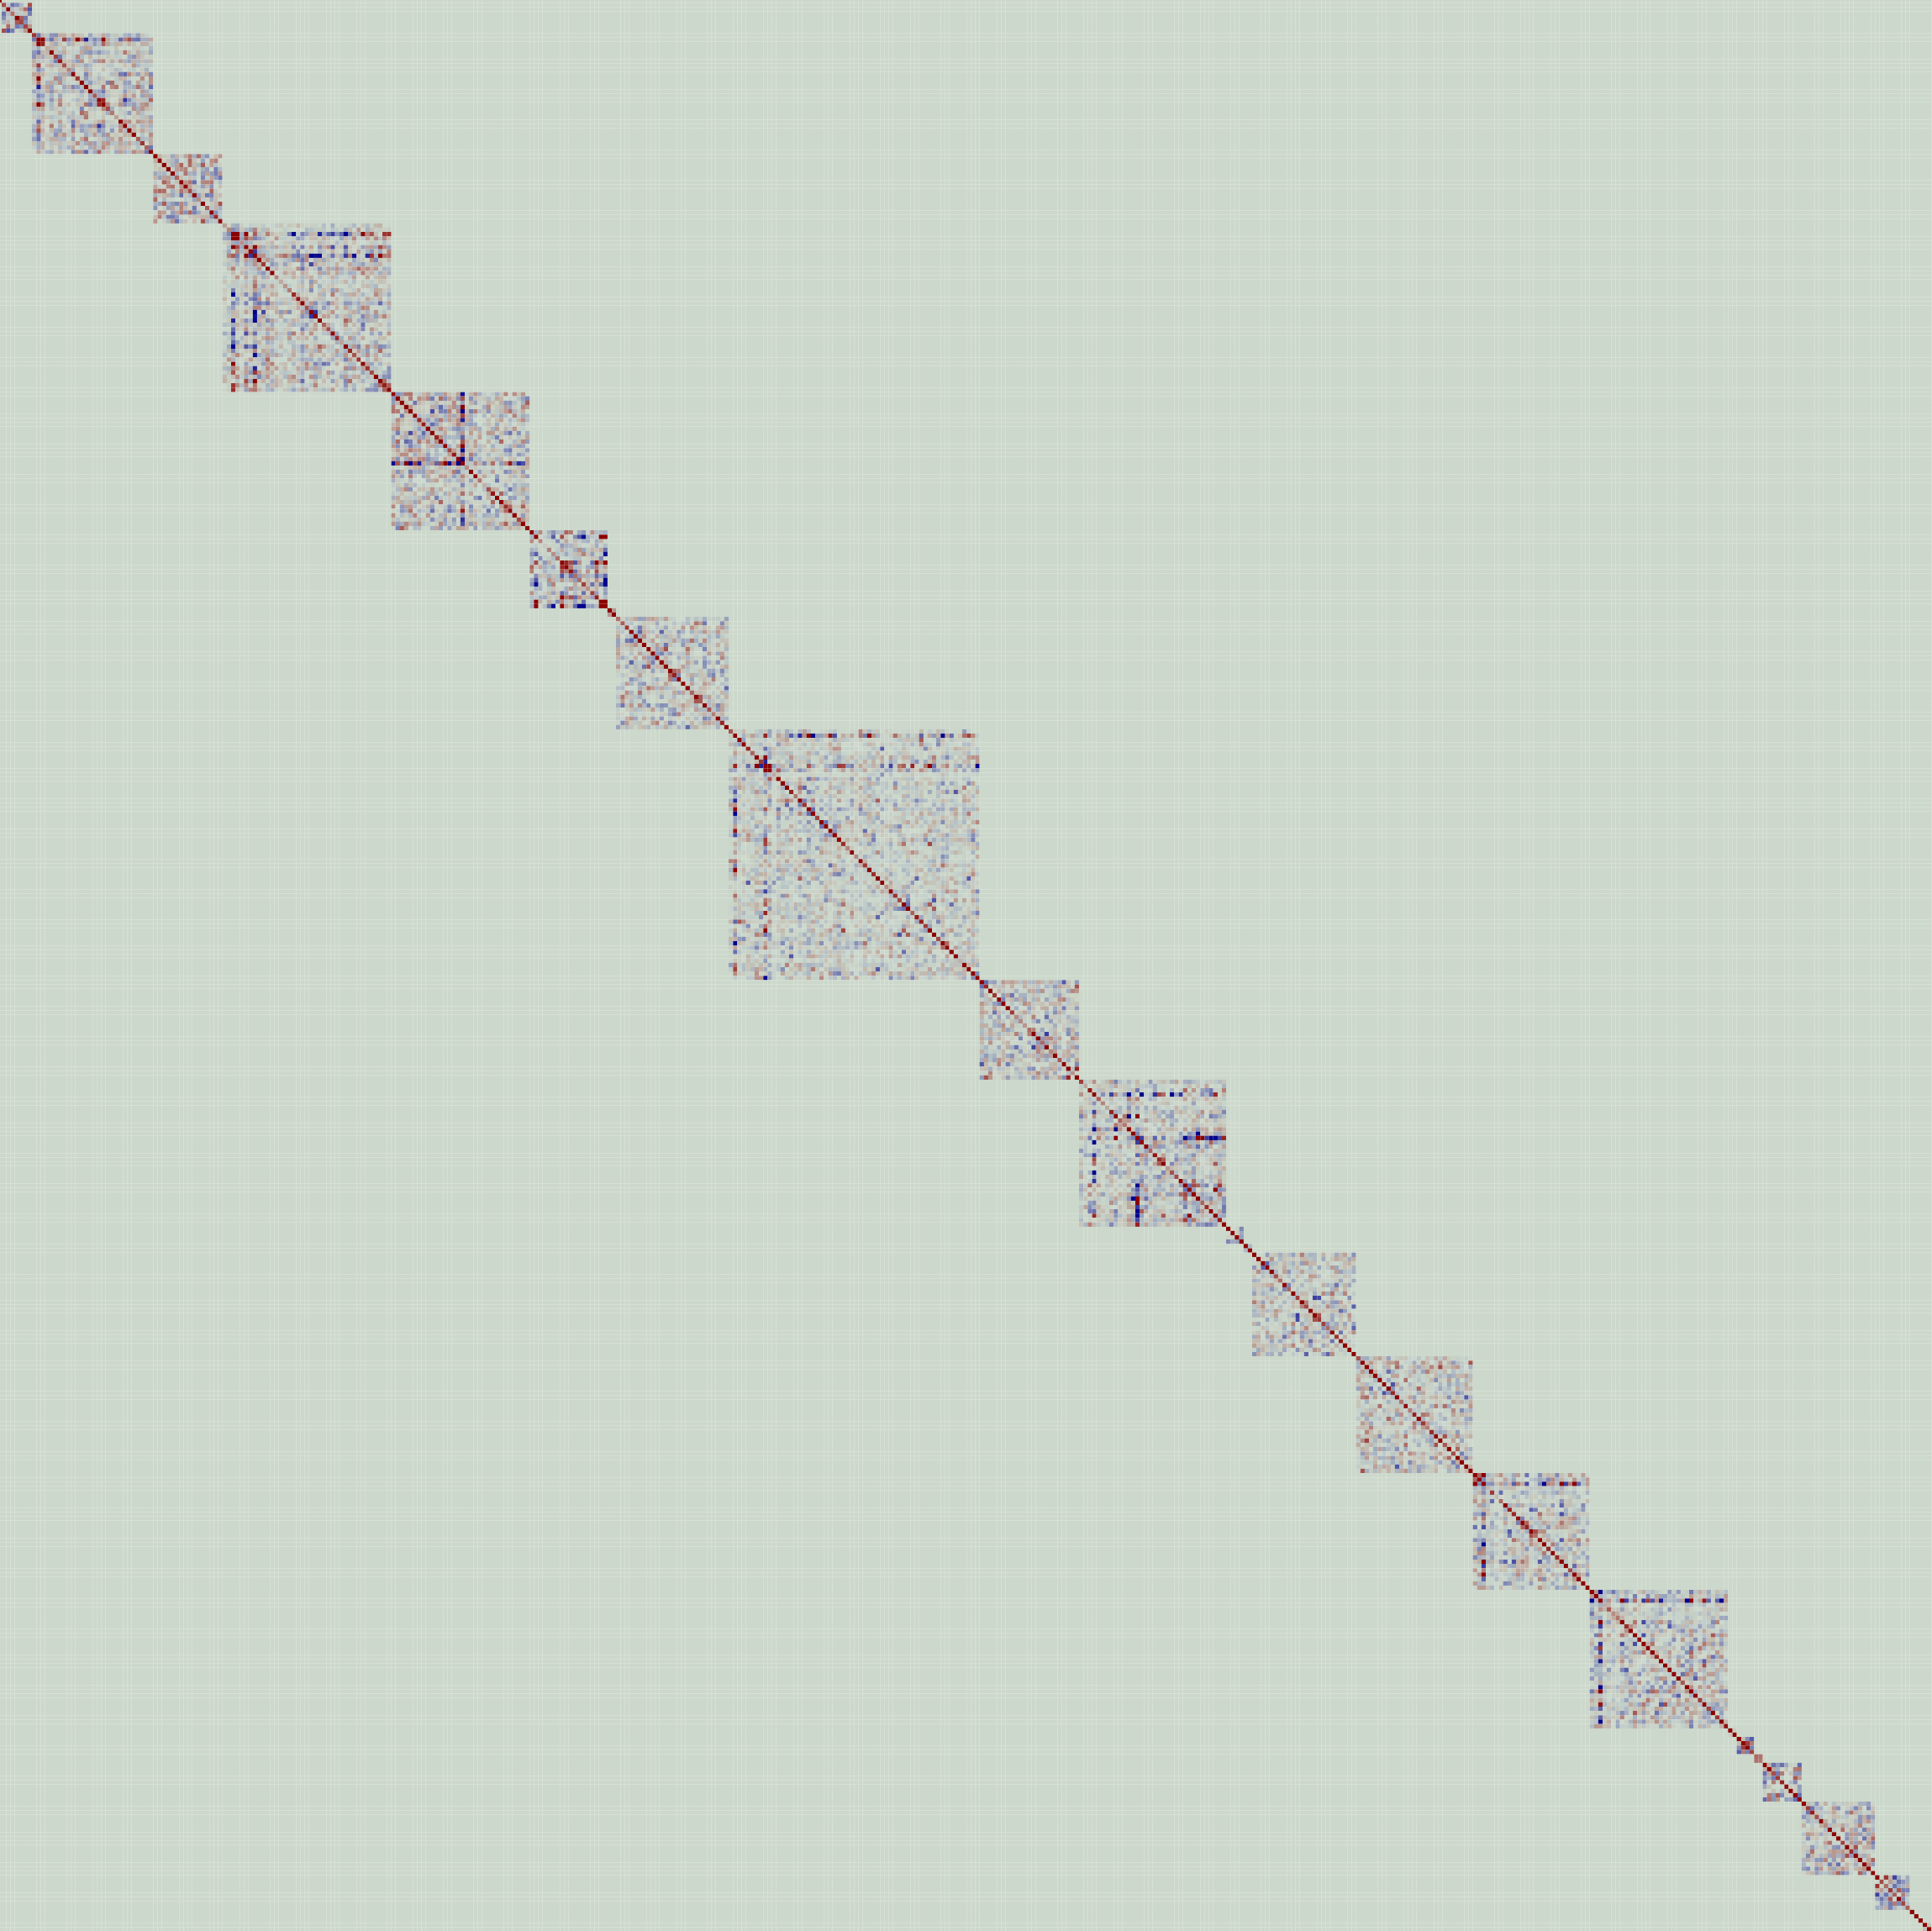
\includegraphics[width=\textwidth]{AutF5_blocks.png}

\end{frame}

\begin{frame}
\centering
\begin{tikzpicture}
\draw [thin, draw=black!20, fill=blue!10] (0,0) grid (10.18,-10.18) rectangle (0,0);
\node at (8, -8.5) {Original sdp constraint};
\node at (.5,-.5) {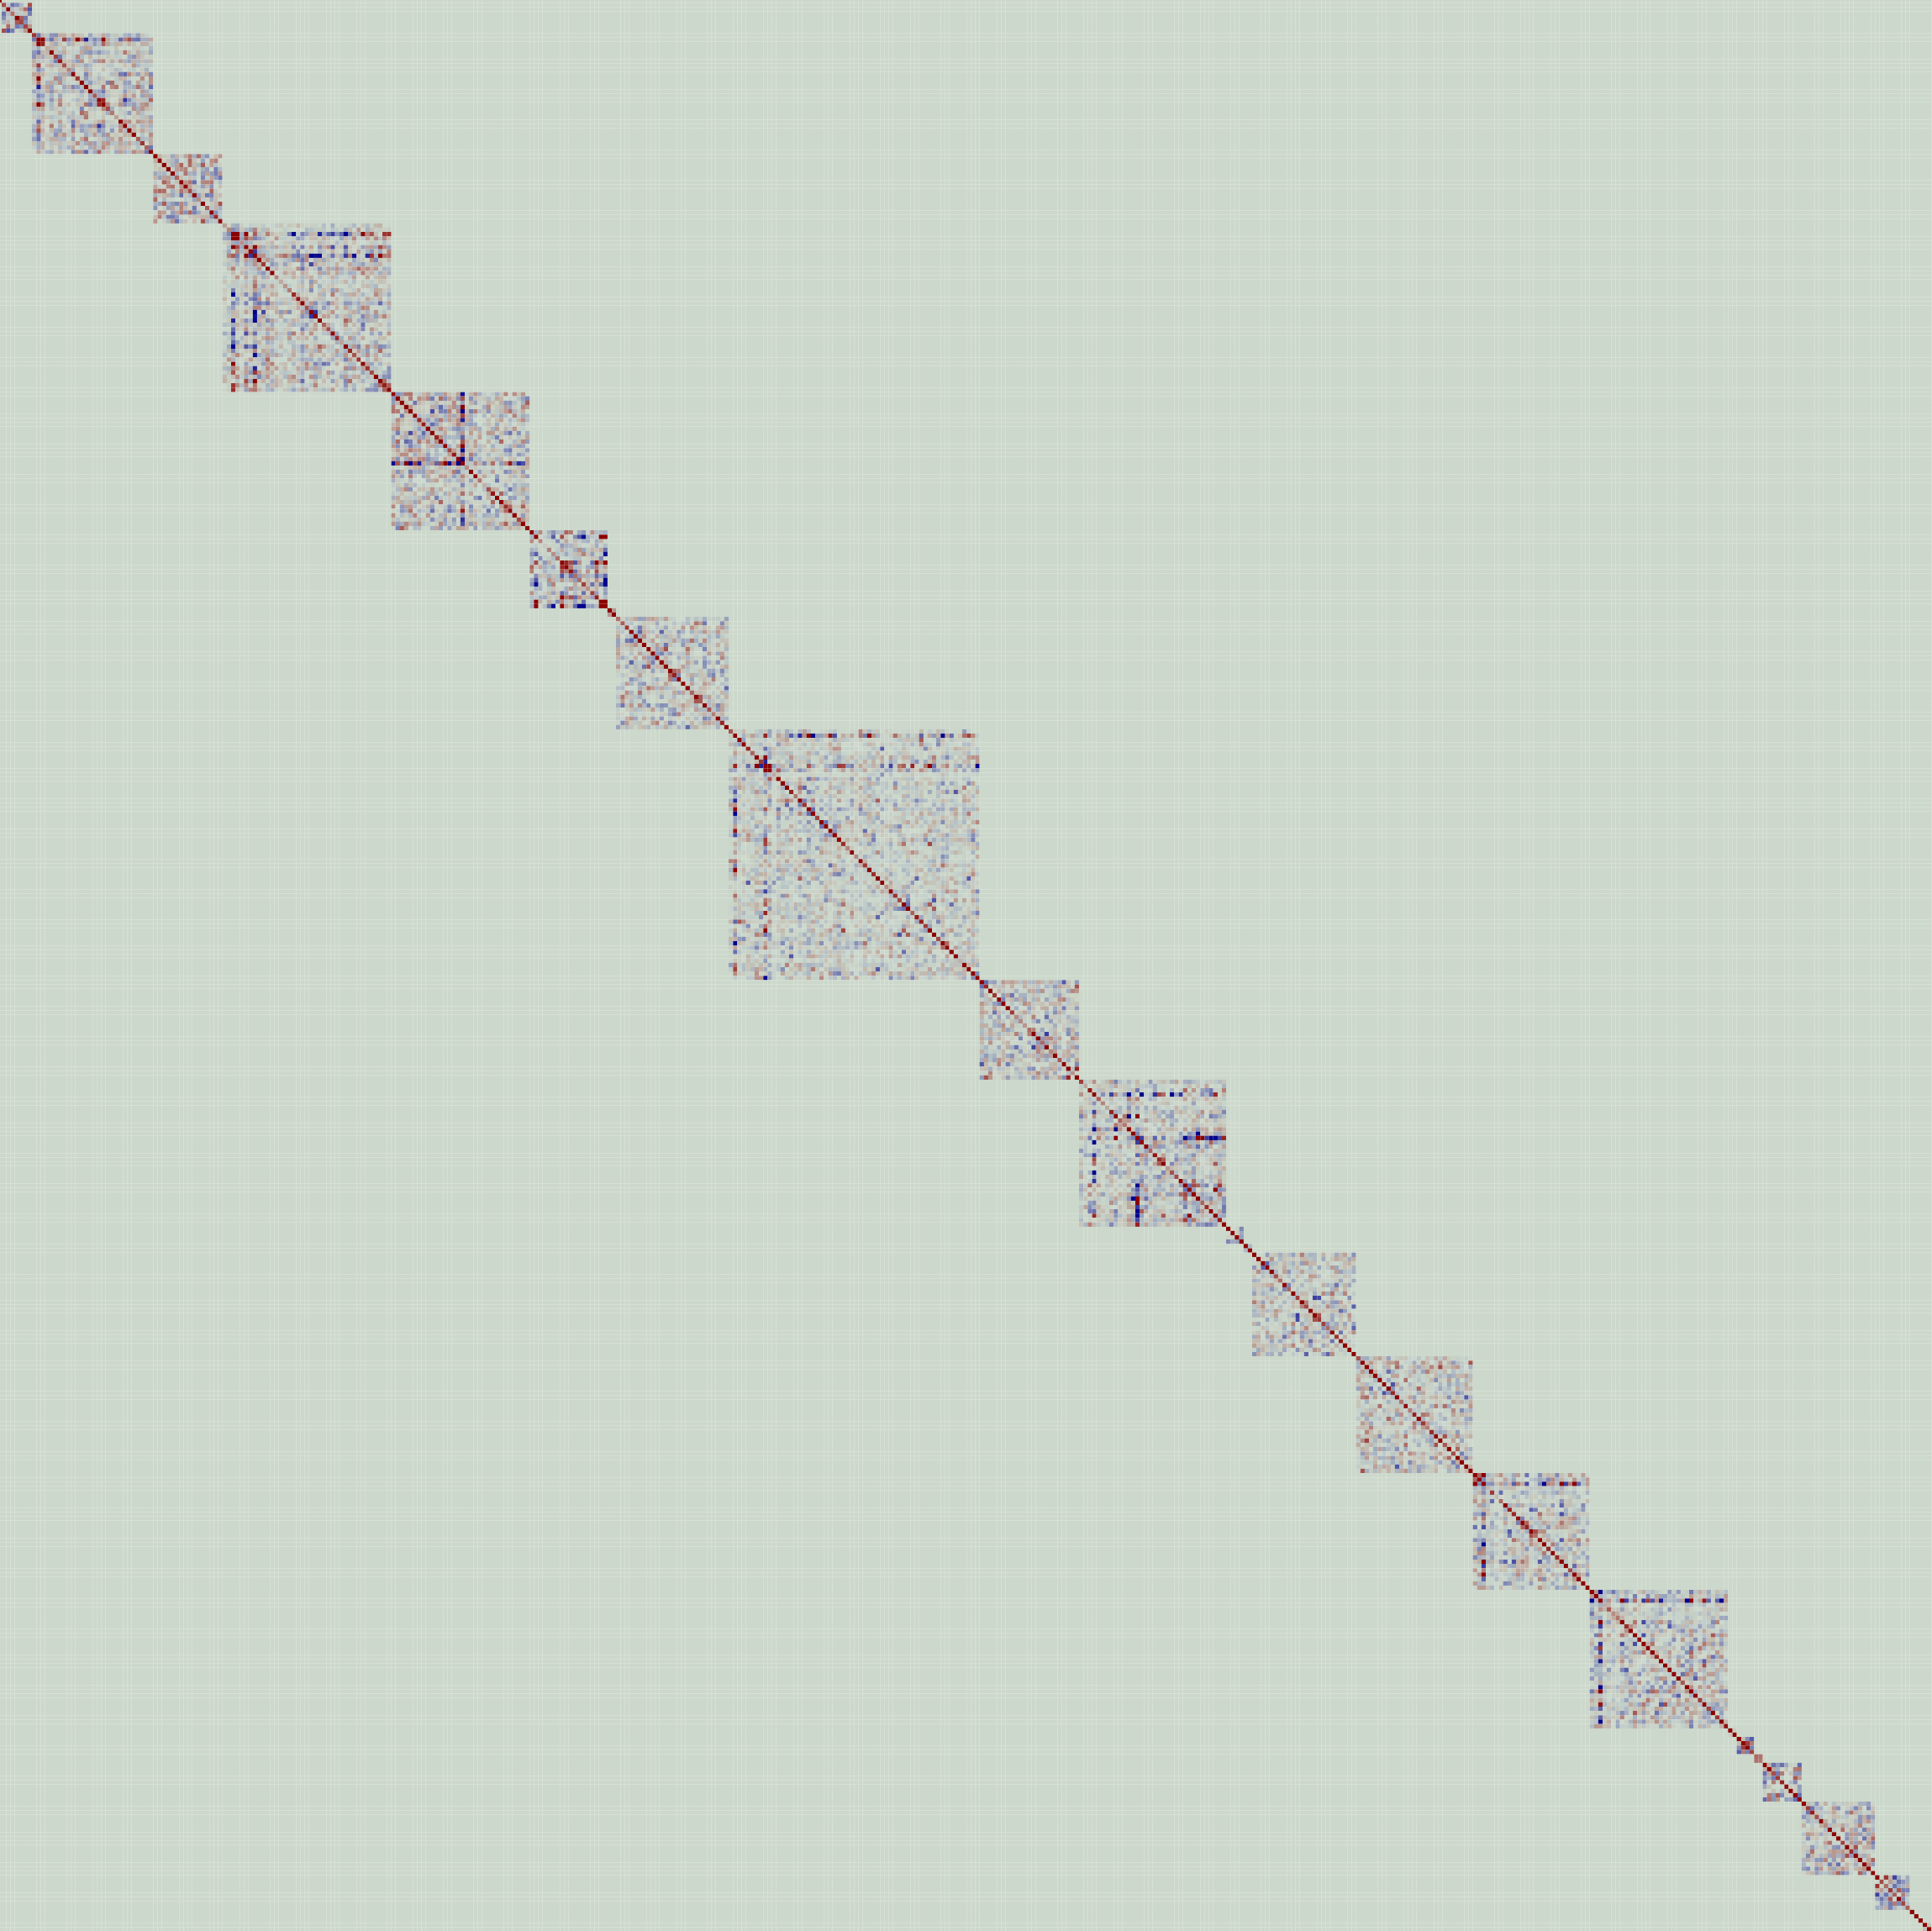
\includegraphics[width=1cm]{AutF5_blocks.png}};

\end{tikzpicture}

\end{frame}




